\chapter{Basic First Aid Principles}\label{ch:basic_principles}

\section{Infection Control and Personal Protection}

Preventing the transmission of disease is a fundamental principle in first aid. Always take precautions to protect both yourself and the person receiving care.

\subsection{Standard Precautions}

Treat all blood and body fluids as potentially infectious. Follow these standard precautions \cite{cdc,who_2018}:

\begin{enumerate}[leftmargin=*]
  \item Wash hands thoroughly with soap and water before and after providing care, or use alcohol-based hand sanitizer (at least 60\% alcohol) if soap and water are unavailable
  \item Wear disposable gloves when there is contact with blood, open wounds, or body fluids
  \item Use protective equipment such as face shields, masks, or goggles when splashing is possible
  \item Avoid direct skin-to-skin contact with open wounds
  \item Dispose of contaminated materials safely in sealed plastic bags
  \item Clean any exposed skin areas immediately with soap and water
\end{enumerate}
\quicknote{\textbf{Glove Usage}: Never reuse disposable gloves. If gloves become torn or punctured during use, remove them immediately and replace with a new pair.}

\section{Assessing Responsiveness}

The first step in any emergency assessment is determining whether the person is conscious and responsive.

\begin{enumerate}[leftmargin=*]
\item Approach the person from the front where they can see you
\item Tap both shoulders firmly and shout loudly: ``Can you hear me? Are you OK?''
\item Look for response: opening eyes, moving, speaking, or following simple commands
\end{enumerate}
\textbf{WARNING:} If there is NO response, call for help immediately and check for breathing and pulse (for unresponsive persons).

\section{Checking Breathing}

For an unresponsive person, checking breathing is critical.

\begin{enumerate}[leftmargin=*]
\item Place your ear near the person's mouth and nose while looking at their chest
\item Listen for breath sounds and feel for air movement on your cheek
\item Look for chest rise and fall over 5-10 seconds
\end{enumerate}
\textbf{WARNING:} If the person is NOT breathing or only gasping abnormally (agonal breaths), assume cardiac arrest and begin CPR immediately.

\section{Checking Pulse}

\textbf{Lay rescuers: do NOT perform a pulse check.} If a person is unresponsive and not breathing normally, assume cardiac arrest and begin CPR immediately -- pulse checks are unreliable in lay hands and delay chest compressions. The pulse check below is for trained or healthcare responders.

The carotid artery (neck) is the most accessible pulse point for adults.

\begin{enumerate}[leftmargin=*]
\item Place two fingers (not your thumb) on the side of the neck, just below the jaw angle
\item Press lightly against the trachea to find the carotid artery
\item Check for a pulse for no more than 10 seconds
\end{enumerate}
\quicknote{\textbf{Children and Infants}: For children up to puberty, use the brachial artery (inner upper arm). For infants (<1 year), also use the brachial artery or femoral artery (groin area).}

\medskip\noindent\textbf{Emergency Summary Table.}
\begin{center}
\begin{tabularx}{\textwidth}{@{}>{\raggedright\arraybackslash}X>{\raggedright\arraybackslash}X>{\raggedright\arraybackslash}X>{\raggedright\arraybackslash}X@{}}
\hline
\textbf{Condition} & \textbf{Response} & \textbf{Breathing} & \textbf{Action} \\
\hline
Responsive & Yes & Normal & Monitor, comfort, seek help if needed \\
Unresponsive & No & Normal & Place in recovery position, monitor continuously \\
Unresponsive & No & Not breathing/Only gasping & Begin CPR immediately (start compressions) \\
\hline
\end{tabularx}
\end{center}

\section{Positioning Unconscious Persons}

Proper positioning helps maintain airway patency and prevents aspiration.

\subsection{Recovery Position (Lateral Recumbent Position)}\label{sec:recovery_position}

Use this position for unconscious but breathing individuals to prevent choking on vomit or secretions.

\begin{enumerate}[leftmargin=*]
\item Kneel beside the person and extend their arm away from you at a right angle
\item Bend their other elbow and place the back of their hand against your cheek
\item Bring their far leg and bend it at the knee
\item Carefully roll them toward you using the bent leg as a pivot point
\item Tilt the head back slightly to keep the airway open
\item Ensure the top leg remains bent to stabilize the position
\end{enumerate}
\begin{figure}[h]
\centering
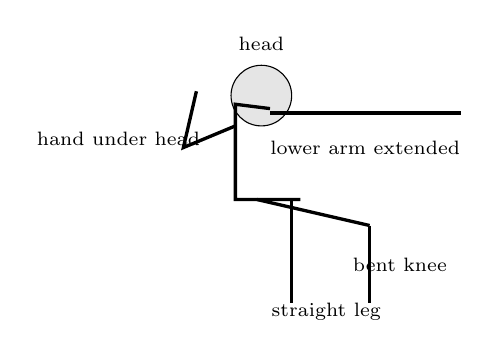
\begin{tikzpicture}[scale=1.1, >=stealth]
  \draw[fill=black!10] (0,0) circle (0.35);
  \node at (0,0.6) {\scriptsize head};
  \draw[very thick] (0.1,-0.2) -- (2.3,-0.2);
  \node at (1.2,-0.6) {\scriptsize lower arm extended};
  \draw[very thick] (0.1,-0.15) -- (-0.3,-0.1) -- (-0.3,-1.2) -- (0.45,-1.2);
  \draw[very thick] (-0.3,-0.35) -- (-0.9,-0.6) -- (-0.75,0.05);
  \node at (-1.65,-0.5) {\scriptsize hand under head};
  \draw[very thick] (0.35,-1.2) -- (0.35,-2.4);
  \node at (0.75,-2.5) {\scriptsize straight leg};
  \draw[very thick] (-0.05,-1.2) -- (1.25,-1.5);
  \draw[very thick] (1.25,-1.5) -- (1.25,-2.4);
  \node at (1.6,-1.95) {\scriptsize bent knee};
\end{tikzpicture}
\caption{Recovery position (viewed from above). The lower arm is extended on the ground, the upper arm's hand is tucked under the head, the near leg is straight, and the far leg is bent at the knee for stability.}
\label{fig:recovery_position}
\end{figure}

\textbf{WARNING:} Do NOT use the recovery position if you suspect spinal injury unless the person is vomiting or not breathing. In suspected spinal injuries, maintain manual in-line stabilization of the head and neck.

\section{Wound Assessment and Basic Care}

All wounds should be assessed quickly and systematically.

\subsection{Types of Wounds}

\begin{description}
  \item[Abrasion:] Scrape or raw surface caused by friction (road rash) that removes the outer layer of skin
  \item[Avulsion:] Partial or complete tearing away of skin and tissue
  \item[Contusion:] Bruise with intact skin but damaged underlying tissues
  \item[Laceration:] Cut or tear through skin and underlying tissue, often jagged edges
  \item[Puncture:] Small, deep wound caused by pointed objects (nails, needles, animal bites)
\end{description}

\subsection{Wound Management Steps}

\begin{enumerate}[leftmargin=*]
\item Ensure personal protection (wear gloves)
\item Control bleeding by applying direct pressure to the wound
\item Clean gently around the wound with sterile saline or clean water (avoid putting hydrogen peroxide or alcohol directly in the wound as it damages tissue)
\item Cover with a sterile dressing or bandage
\item Monitor for signs of infection (increased redness, warmth, swelling, pus, fever)
\end{enumerate}
\textbf{WARNING:} Seek immediate medical attention for: deep puncture wounds, animal/bite wounds, dirty wounds not cleaned within 8 hours, wounds with embedded objects, or signs of systemic infection.

\section{Basic Bandaging Techniques}

Proper bandaging supports healing without cutting off circulation.

\subsection{Glass Cuts}

Glass produces sharp, often clean lacerations that can be deeper than they appear. Special considerations include embedded fragments, tetanus risk, and stitch requirements.

\subsubsection{Initial Assessment}

\begin{itemize}[leftmargin=*]
  \item Assess bleeding severity — glass cuts may bleed steadily even if not spurting
  \item Look for visible glass fragments — use bright light and magnification if available
  \item Check depth — if the cut is deep enough to see fat, muscle, tendon, or bone, or if edges are gaping widely, seek medical evaluation for possible stitches
  \item Ask about tetanus vaccination status — a booster is recommended if the last shot was more than 5 years ago for dirty wounds like glass
\end{itemize}

\subsubsection{Managing Small Surface Fragments}

If small, visible glass fragments sit on the surface or just under the skin:

\begin{enumerate}[leftmargin=*]
  \item Wash your hands thoroughly and use clean tweezers (cleaned with alcohol if available)
  \item Gently lift or slide the fragment out in the direction it entered — do not dig deeply or enlarge the wound
  \item If the fragment is deeply embedded or you cannot remove it easily, DO NOT force it — cover with a sterile dressing and seek medical care
\end{enumerate}
\subsubsection{Wound Care After Fragment Removal}

\begin{enumerate}[leftmargin=*]
  \item Rinse the wound thoroughly with clean running water for several minutes to flush out any remaining tiny particles
  \item Clean gently around the wound with mild soap (avoid getting soap directly in the wound)
  \item Apply an over-the-counter antibiotic ointment (e.g., bacitracin or neomycin)
  \item Cover with a sterile adhesive bandage or non-stick dressing
  \item Change the dressing daily or whenever it becomes wet or soiled
\end{enumerate}
\subsubsection{When to Seek Medical Attention}

Seek professional care if:
\begin{itemize}[leftmargin=*]
  \item Bleeding continues after 10-15 minutes of steady direct pressure
  \item The wound is deeper than 1/4 inch (6 mm) or is gaping open
  \item You cannot remove all glass fragments
  \item Signs of infection develop (increasing redness, warmth, swelling, pus, fever)
  \item Numbness, tingling, or inability to move fingers/toes near the injury (possible nerve/tendon damage)
  \item The cut is on the face, hands, feet, or joints where precise closure matters
  \item Tetanus vaccination is unknown or outdated
\end{itemize}

\noindent\textbf{Note}: Unlike impaled glass (see Chapter~\ref{ch:bleeding}, Section~\ref{sec:embedded_objects}, "Embedded Objects"), surface glass cuts should generally have visible fragments carefully removed when possible, followed by thorough cleaning and appropriate wound care.


\subsection{Wrap Technique}

Apply gauze wraps with light tension, overlapping each turn by one-half to two-thirds. Check circulation distal to the bandage (color, temperature, sensation, capillary refill every 15 minutes).

\subsection{Triangular Sling}

Used to support injured arms or shoulders. Form a triangle with cloth, place the arm across the body, tie knots at the neck behind the ear, and tuck the tip of the sling under the elbow.

\textbf{WARNING:} Check frequently for impaired circulation: pale fingers, coldness, numbness, tingling, or inability to move fingers. Loosen immediately if any occur.

\section{Temperature Control}

Maintaining normal body temperature is crucial in emergencies.

\subsection{Hypothermia (Low Body Temperature)}

\begin{itemize}[leftmargin=*]
  \item Shivering, slurred speech, coordination problems, drowsiness
  \item Move to warm environment, remove wet clothing
  \item Cover with dry blankets, warm from the trunk outward (use body heat or warm packs on chest, neck, groin, and armpits -- NOT extremities)
  \item Offer warm sweet liquids if the person is alert and able to swallow
  \item Do NOT give alcohol or caffeine
  \item Seek medical assistance promptly
\end{itemize}

\subsection{Hyperthermia (High Body Temperature)}

Heat exhaustion: heavy sweating, weakness, nausea, cool/moist skin, rapid pulse. Move to cool place, rest, drink cool water, apply cool wet cloths, loosen clothing.

Heat stroke (medical emergency): body temperature >104°F (40°C), hot/dry skin or profuse sweating, confusion, loss of consciousness. CALL EMERGENCY SERVICES IMMEDIATELY. Cool the person rapidly with any available means (cold water immersion, wet cloths, ice packs on neck/armpits/groin).

\section{Key Takeaways}

\medskip\noindent\textbf{First Aid Safety Checklist.}
\begin{itemize}
  \item Ensure scene safety before approaching
  \item Assess responsiveness and breathing
  \item Call emergency services when needed
  \item Protect yourself and others from infection
  \item Position unconscious breathing persons properly
  \item Control bleeding with direct pressure
  \item Monitor for changes in condition continuously
\end{itemize}

\section{Review Questions}

\begin{enumerate}[leftmargin=*]
\item List four standard precautions that protect both you and the person you are helping.
\item How do you check an unresponsive person's breathing, and for how long?
\item When is the recovery position used, and when should it be avoided?
\item How long must continuous direct pressure be applied before checking whether bleeding has stopped?
\item Why should hydrogen peroxide or alcohol not be poured directly into a wound?
\end{enumerate}
\section{Skill Practice: Basic Response}

Use this checklist to practice with a partner and confirm each step before it becomes routine.

\begin{enumerate}[leftmargin=*]
\item Check scene safety; state any hazards you find
\item Put on disposable gloves correctly
\item Tap and shout to check responsiveness
\item Call for help (simulate) and note the time
\item Check breathing for 5--10 seconds (look, listen, feel)
\item Demonstrate the recovery position, then return the person to supine safely
\item Control simulated bleeding with a dressing and firm pressure for 5 minutes
\item Check pulse and capillary refill distal to a bandage
\item Reassess the person and report your observations as if to a responder
\end{enumerate}
\index{infection control}
\index{personal protection}
\index{responsiveness assessment}
\index{breathing check}
\index{pulse assessment}
\index{recovery position}
\index{wound management}
\index{bandaging techniques}
\index{hypothermia treatment}
\index{hyperthermia treatment}